\chapter{Conceção e Desenvolvimento}
\label{cp:concecao-implementacao}

Este capítulo descreve a arquitetura geral do \textit{Plot in a Pot}, detalhando as decisões de design de dados, o funcionamento dos algoritmos de processamento, as estratégias de visualização e acessibilidade adotadas, e o motor de simulação implementado.

\section{Arquitetura Geral do Sistema}
\label{sec:arquitetura-geral}
O sistema foi desenhado segundo uma arquitetura modular dividida em três camadas conceptuais independentes de tecnologia. Esta abordagem garante a separação de responsabilidades entre a recolha de comandos, o processamento de dados e a sua persistência, promovendo a manutenibilidade e a evolução isolada de cada módulo:
\begin{enumerate}
    \item \textbf{Camada de Apresentação (Interface):} Responsável por gerir a interação direta com o utilizador. É constituída por:
    \begin{itemize}
        \item \textbf{Canvas de Grafos:} O espaço visual interativo onde o autor cria, manipula e liga os nós narrativos.
        \item \textbf{Matriz de Tradução:} Uma grelha estruturada que expõe os dicionários de localização e permite a tradução de chaves de texto em tempo real.
        \item \textbf{Ecrã do Simulador:} A interface interativa de jogo onde o autor testa e experimenta a narrativa sob o ponto de vista do leitor.
    \end{itemize}
    \item \textbf{Camada de Processamento Lógico (Núcleo):} Contém a inteligência do sistema e os motores de transformação. É constituída por:
    \begin{itemize}
        \item \textbf{Parser Twee 3:} Módulo encarregue de ler ficheiros de texto estruturados em formato Twee 3 e convertê-los no modelo interno da aplicação, bem como serializar e exportá-los de volta.
        \item \textbf{Validador Estático:} Motor que executa travessias de grafo (\gls{bfs}/\gls{dfs}) para inspecionar inconsistências estruturais, como ciclos sem saída, nós inacessíveis ou hiperligações quebradas.
        \item \textbf{Motor de Simulação:} Sandbox responsável por inicializar scripts customizados, interpretar condicionais lógicas e controlar o estado de jogo na simulação. Este estado é representado por um conjunto de variáveis lógicas globais e locais que registam as decisões do utilizador (ex: inventário, escolhas de caminhos ou pontuações).
    \end{itemize}
    \item \textbf{Camada de Dados e Persistência:} Representa o modelo de informação e o armazenamento. É constituída por:
    \begin{itemize}
        \item \textbf{Lista de Adjacência:} O modelo de dados em memória que representa a topologia do grafo, as saídas (sucessores) e entradas (predecessores) de cada cena.
        \item \textbf{Dicionários \gls{json}:} A base de dados estruturada que armazena os dicionários de tradução e localização no armazenamento local.
    \end{itemize}
\end{enumerate}

O fluxo de funcionamento da aplicação e a relação de comunicação entre estas camadas encontram-se representados no diagrama detalhado da Figura~\ref{fig:arquitetura-conceptual}.

\begin{figure}[htbp]
\centering
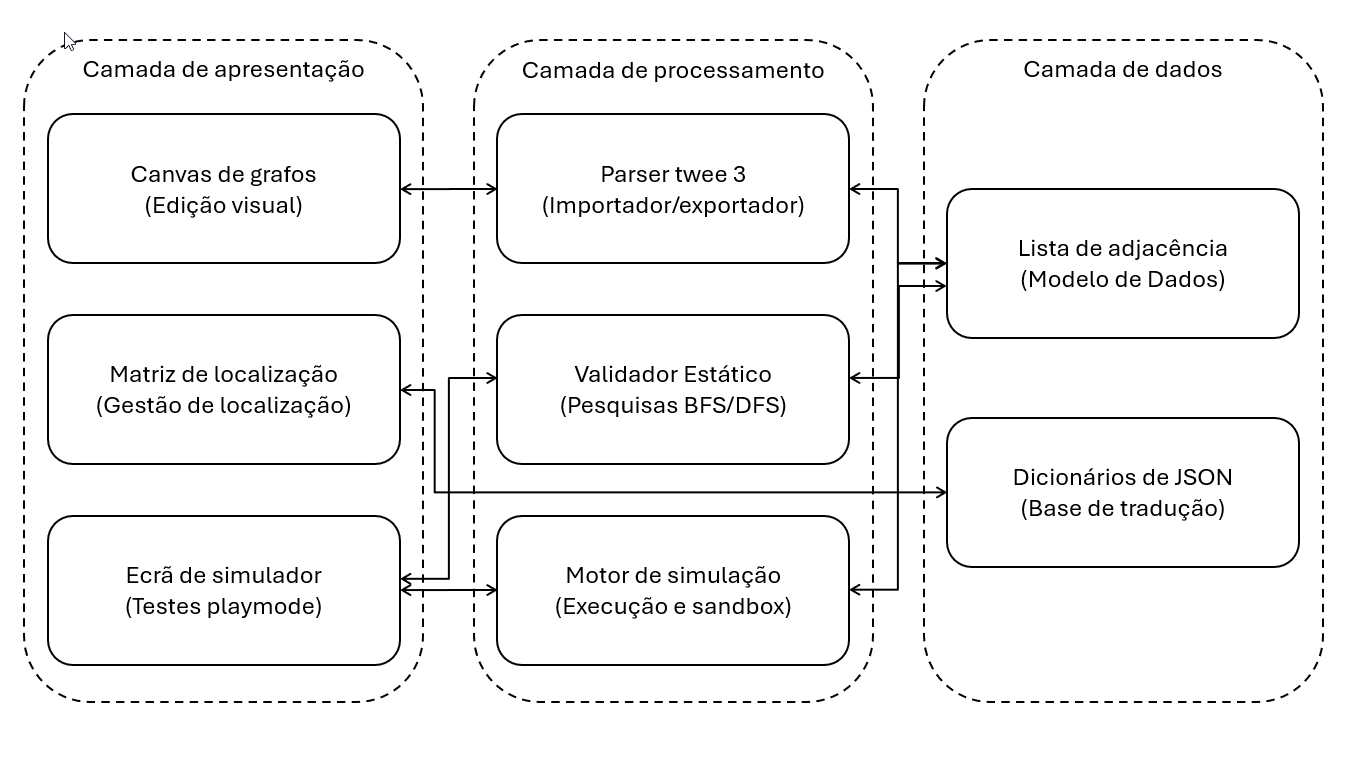
\includegraphics[width=0.9\linewidth]{Figures/arquitetura.png}
\caption{Diagrama de blocos detalhado da arquitetura conceptual e fluxo de dados.}
\label{fig:arquitetura-conceptual}
\end{figure}

\section{Requisitos do Sistema}
\label{sec:requisitos-sistema}

Com o intuito de delimitar o âmbito do projeto, o sistema foi estruturado para responder a necessidades fundamentais de modelação visual, internacionalização nativa, análise estática de integridade e inteligência artificial no cliente. Para a materialização prática do \gls{piap}, estas necessidades foram detalhadas sob a forma de requisitos técnicos, divididos entre funcionais (comportamento direto da aplicação) e não funcionais (restrições de qualidade, desempenho e usabilidade).

\subsection{Requisitos Funcionais}
\begin{description}
    \item[\textbf{RF01 - Criação e Edição de Nós Narrativos (Cenas):}] O utilizador deve poder instanciar, arrastar, atualizar (título e corpo de texto das cenas) e remover de forma atómica nós narrativos no canvas bidimensional.
    \item[\textbf{RF02 - Ligações Direcionadas entre Nós (Escolhas):}] O sistema deve inferir e instanciar arestas direcionadas automaticamente no grafo a partir da análise reativa de hiperligações double-bracket (\texttt{[[Texto|Destino]]}) inseridas pelo autor no texto das passagens.
    \item[\textbf{RF03 - Parser e Compatibilidade Twee 3:}] O sistema deve assegurar a interoperabilidade bidirecional síncrona com a especificação Twee 3, suportando a importação e exportação de ficheiros com extensão \texttt{.twee}, mantendo a sintaxe e efetuando o mapeamento geométrico das coordenadas espaciais dos nós.
    \item[\textbf{RF04 - Auditoria e Validação Estática de Fluxo:}] A plataforma deve executar análises estáticas e reativas sobre a topologia do grafo em plano secundário, sinalizando inconsistências estruturais como nós órfãos (inacessíveis), becos sem saída (hiperligações para identificadores inexistentes) ou caminhos inacessíveis devido a restrições lógicas.
    \item[\textbf{RF05 - Matriz de Localização Multi-idioma:}] O sistema deve disponibilizar uma matriz de tradução tabular centralizada que associe chaves dinâmicas das passagens a múltiplos dicionários de tradução, permitindo a exportação e importação síncrona de ficheiros em formato \gls{csv} em conformidade com a norma RFC 4180.
    \item[\textbf{RF06 - Simulador em Tempo Real (PlayMode):}] A aplicação deve integrar um simulador interativo em tempo real (\textit{PlayMode}) executado sob uma sandbox isolada do DOM, interpretando macros SugarCube, avaliando condições lógicas e executando scripts ou estilos customizados.
    \item[\textbf{RF07 - Zonas de Agrupamento Visual:}] O utilizador deve ser capaz de delimitar contêineres espaciais redimensionáveis (Zonas) para agrupamento lógico e organização de nós de cena, permitindo a sua translação conjunta no canvas.
    \item[\textbf{RF08 - Importação Inteligente via Conversor LLM:}] O sistema deve disponibilizar um assistente de inteligência artificial capaz de converter narrativas lineares em linguagem natural para o formato estruturado Twee 3, recorrendo à integração assíncrona com modelos de linguagem locais (Ollama) ou APIs externas.
\end{description}

\subsection{Requisitos Não Funcionais}
\begin{description}
    \item[\textbf{RNF01 - Portabilidade e Execução no Cliente (Browser):}] A plataforma deve ser executável inteiramente no lado do cliente através de um navegador de internet padrão, sem requerer servidores ou infraestruturas complexas.
    \item[\textbf{RNF02 - Usabilidade e Acessibilidade Visual:}] A interface de grafos deve utilizar a estética neo-brutalista e garantir que a visualização de fluxos (arestas de entrada e saída) seja distinguível sem dependência exclusiva de cor, apoiando utilizadores daltónicos.
    \item[\textbf{RNF03 - Desempenho e Fluidez:}] O canvas do React Flow e a conversão do parser síncrono devem suportar dezenas de nós em simultâneo com latência de interação e atualização abaixo de 100 milissegundos.
    \item[\textbf{RNF04 - Privacidade e Soberania de Dados:}] Todos os dados introduzidos, incluindo ficheiros importados, tabelas de tradução e dados submetidos para inteligência artificial no Ollama local, devem permanecer estritamente no armazenamento local do utilizador para garantir segurança absoluta.
\end{description}

\section{Métodos, Técnicas e Enquadramento Tecnológico}
\label{sec:metodos-tecnologia}

Para concretizar as especificações da arquitetura conceptual e responder aos requisitos definidos, o projeto apoia-se em metodologias ágeis de prototipagem rápida e numa seleção de tecnologias executadas do lado do cliente. As principais opções metodológicas e técnicas encontram-se estruturadas a seguir:

\begin{itemize}
    \item \textbf{Desenvolvimento da SPA (React 19) e Estilização (Tailwind CSS 3):}
    A aplicação foi inteiramente estruturada e programada pela equipa como uma \gls{spa} em \textbf{React 19} \citep{ReactReference}, tirando partido da nossa experiência prévia com esta tecnologia para gerir reativamente a árvore de componentes da interface. A identidade visual neo-brutalista (de alto contraste e bordas sólidas) foi desenhada e implementada por nós através da aplicação de classes utilitárias de \textbf{Tailwind CSS 3} \citep{TailwindCSSReference} nos componentes do editor.

    \item \textbf{Extensões ao Canvas de Grafos (ReactFlow 11):}
    Em vez de desenvolvermos um motor de desenho vetorial do zero, utilizámos a biblioteca \textbf{ReactFlow 11} \citep{ReactFlowReference} como base para gerir interações de zoom e arrasto. O nosso trabalho consistiu em estender esta infraestrutura básica através do desenvolvimento de nós totalmente customizados de cena (\texttt{StoryNode.jsx}) e de agrupamento (\texttt{ZoneNode.jsx}), além de arestas interativas personalizadas.

    \item \textbf{Algoritmia de Validação (Teoria de Grafos):}
    Concebemos e implementámos um modelo de dados baseado em listas de adjacências bidirecionais locais. Sobre esta estrutura, programámos algoritmos específicos para realizar análises topológicas em plano secundário (deteção de inconsistências via BFS) e a simulação de caminhos heurística do \textit{Smart Walker}.

    \item \textbf{Sistema de Internacionalização (i18next):}
    Integrámos a biblioteca \textbf{i18next} para gerir dicionários locais. Desenvolvemos o mapeamento que associa os dados tabulares da matriz de tradução do utilizador a ficheiros JSON de localização estáticos, carregados dinamicamente no navegador com o plugin de cliente \texttt{i18next-http-backend} sob o modelo \textit{backendless}.
\end{itemize}

\subsection{Justificação das Decisões de Design}
\label{subsec:justificacao-decisoes-design}
Com base na análise comparativa das ferramentas existentes (ver Secção~\ref{sec:analise-comparativa}), as escolhas de design e de tecnologia para o \gls{piap} foram fundamentadas nos seguintes pontos:
\begin{itemize}
    \item \textbf{Fusão de Paradigmas (Visual vs. Textual):} Enquanto o Twine se destaca pela interface puramente visual e o Ink pelo controlo fino de estados lógicos complexos, o \gls{piap} visa fundir ambas as forças, proporcionando um editor visual de grafos que não abdica da manipulação robusta de condicionais e variáveis (via macro-linguagem SugarCube).
    \item \textbf{Adoção do Formato Aberto Twee 3 e Limitação de Grafos:} A especificação aberta Twee 3 possui um mapeamento direto entre passagens e grafos, o que suporta a decisão de adotá-lo como base de persistência do \gls{piap}. Contudo, para permitir que o sistema leia as saídas e as renderize visualmente como arestas de forma fiável, o projeto introduz um compromisso de design (\textit{trade-off}) em relação ao Twine tradicional: não é suportada a utilização de variáveis como destinos dinâmicos de hiperligações (ex: \texttt{[[Ir para o local|\$local]]}), exigindo que todos os destinos do grafo sejam estáticos (conforme detalhado na Secção~\ref{subsec:destinos-dinamicos}).
    \item \textbf{Validação Automática e Segurança do Fluxo:} O ChoiceScript é valorizado pelas suas ferramentas robustas de teste automático (\texttt{randomtest}), uma lacuna crítica do Twine. O \gls{piap} incorpora de raiz este princípio ao disponibilizar o validador estático (\gls{bfs}) e o Smart Walker no simulador para preencher esta falta, garantindo a correção imediata do fluxo narrativo.
    \item \textbf{Autonomia e Licenciamento Livre:} A restrição de uso comercial imposta pelo ChoiceScript salienta a importância de desenvolver uma ferramenta que promova a autonomia dos autores, permitindo a exportação de projetos sob licenças livres e sem taxas adicionais.
\end{itemize}

\section{Modelação de Dados: Lista de Adjacência}
Para representar o fluxo da história no editor, o sistema utiliza uma \textbf{Lista de Adjacência Bidirecional}. Cada cena no modelo de dados armazena de forma independente dois conjuntos de caminhos:
\begin{itemize}
    \item \textbf{Saídas (Sucessores):} Um vetor que contém as escolhas explícitas disponíveis para o leitor, mapeando o texto da opção e o ID do nó de destino.
    \item \textbf{Entradas (Predecessores):} Um vetor que regista as referências de todos os outros nós que contêm escolhas a apontar para o nó atual.
\end{itemize}

Esta representação permite à aplicação realizar o mapeamento reverso instantâneo (\textit{backward mapping}), alimentando os painéis ``Vens de...'' e ``Vais para...'' na interface. A estrutura de dados \gls{json} representativa de um nó apresenta o seguinte formato simplificado:

\begin{code}
{
  "id": "cena_praca",
  "titulo": "A Praça Central",
  "conteudo": "O sol brilha no mercado central.",
  "saidas": [
    { "texto_escolha": "Entrar na taberna", "destino": "cena_taberna" }
  ],
  "entradas": ["cena_taberna"]
}
\end{code}

Note-se que este modelo foca-se exclusivamente na estrutura topológica do grafo. As variáveis globais e as condições lógicas SugarCube não são serializadas na lista de adjacências, sendo integradas diretamente no corpo de texto (\texttt{conteudo}) das passagens e interpretadas em tempo de execução pelo simulador.

\section{Parser Síncrono e Especificação Twee 3}
O ficheiro \texttt{tweeParser.js} (localizado em \texttt{/src/utils/tweeParser.js}) trata da sincronização bidirecional em tempo real entre o canvas do React Flow e o formato de texto Twee 3 \citep{Twee3Reference}.

Esta sincronização acontece de forma síncrona diretamente na memória do navegador. Isto significa que qualquer alteração de coordenadas, edição de texto ou criação de novas ligações no canvas é traduzida de imediato para a estrutura Twee 3 interna (e o oposto também se verifica), sem tempos de espera ou passos de compilação. Como a ferramenta funciona inteiramente no lado do cliente (\textit{client-side}), este mapeamento apenas mantém o estado da sessão atualizado; a persistência física dos dados no disco rígido requer sempre que o utilizador exporte o ficheiro de forma explícita.

\subsection{Importação e Conversão de Coordenadas de Zonas}
\label{subsec:conversao-coordenadas-zonas}
Durante a leitura e escrita de ficheiros, o parser converte as coordenadas de posição absolutas guardadas no formato Twee 3 (explicadas na Secção~\ref{subsec:metadados-tags-twee}) em coordenadas locais quando um nó é filho de uma Zona(explicado na Secção~\ref{subsec:zonas-agrupamento}). O React Flow exige que os nós filhos tenham posições relativas ao canto superior esquerdo da zona mãe, calculadas por:
\[
X_{\text{relativo}} = X_{\text{absoluto}} - X_{\text{zona}}
\]
\[
Y_{\text{relativo}} = Y_{\text{absoluto}} - Y_{\text{zona}}
\]
No processo inverso de exportação para ficheiro \texttt{.twee}, o parser executa a conversão inversa para manter a compatibilidade com outros compiladores de Twine:
\[
X_{\text{absoluto}} = X_{\text{zona}} + X_{\text{relativo}}
\]
\[
Y_{\text{absoluto}} = Y_{\text{zona}} + Y_{\text{relativo}}
\]

\subsection{Passagens Especiais}
O parser reconhece passagens reservadas de metadados da especificação Twee 3:
\begin{itemize}
    \item \texttt{:: StoryTitle}: Define o título do projeto.
    \item \texttt{:: StoryData}: Contém as configurações globais em formato \gls{json}, incluindo o identificador único da história (\texttt{ifid}), o formato de compilação (\texttt{SugarCube}), o nó de arranque (\texttt{start}) e o nível de zoom.
    \item \texttt{:: StoryInit}: Nó especial não-narrativo onde são declaradas e inicializadas as variáveis lógicas de controlo do estado da simulação (as quais servem de memória do jogo, conforme introduzido na Secção~\ref{sec:arquitetura-geral}).
\end{itemize}

\subsection{Modelo SugarCube (Ligações e Macros)}
As arestas são extraídas do texto narrativo de cada nó através de expressões regulares que identificam ligações no formato clássico Twee:
\begin{itemize}
    \item \textbf{Arestas Simples:} \texttt{[[Cena2]]}
    \item \textbf{Arestas com Alias ou Direcionamento:} \texttt{[[Ir para a Taverna|cena\_taberna]]} ou \texttt{[[Abrir porta->cena\_interior]]}
\end{itemize}

No caso das macros de alteração de estado (ex: \texttt{<<set \$moedas += 10>>}) e condicionais lógicas (ex: \texttt{<<if \$tem\_chave>> ... <</if>>}), o parser de importação não as compila nem as remove do texto. O parser executa duas operações:
\begin{enumerate}
    \item \textbf{Preservação de Código:} Mantém as macros intactas no corpo textual da passagem, permitindo que sejam interpretadas e executadas reativamente pelo simulador (\textit{PlayMode}) durante a execução do jogo (ver Secção~\ref{subsec:compilador-jit-macros}).
    \item \textbf{Extração de Variáveis para Indexação:} Identifica os nomes das variáveis (iniciadas por \texttt{\$}) e regista-as no painel de gestão de variáveis, permitindo que o autor as rastreie ou renomeie de forma atómica em todo o projeto.
\end{enumerate}

\section{Interação Visual, Edição e Acessibilidade}

\subsection{Zonas de Agrupamento Visual}
\label{subsec:zonas-agrupamento}
As \textbf{Zonas de Agrupamento Visual} (\texttt{ZoneNode}) consistem em contentores espaciais retangulares que agrupam logicamente nós de cena relacionados (como capítulos ou localizações), conforme ilustrado na Figura~\ref{fig:exemplo-zona}.

\begin{figure}[H]
    \centering
    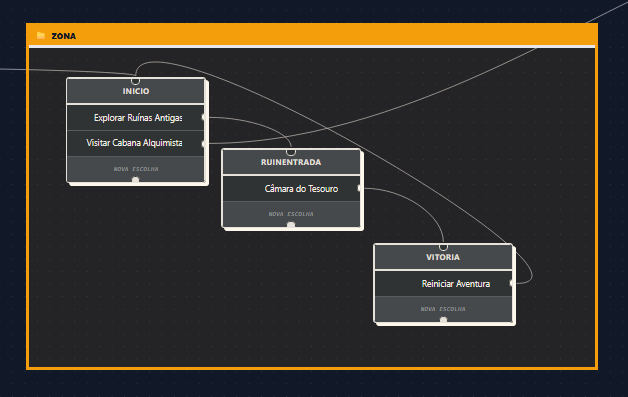
\includegraphics[width=0.65\textwidth]{Figures/zone.png}
    \caption{Exemplo de uma Zona de Agrupamento Visual com nós de cena filhos no canvas.}
    \label{fig:exemplo-zona}
\end{figure}

A sua implementação como nós de grupo personalizados exigiu contornar um problema de colisão de cliques no React Flow. Como o contentor cobre uma área retangular considerável sobreposta aos nós de cena interiores, os \textit{pointer events} capturavam os cliques no ecrã, impedindo a seleção ou arrasto dos filhos. Para resolver isto, definiu-se a propriedade CSS \texttt{pointer-events: none} dinamicamente na configuração global do React Flow para o contentor da Zona em \texttt{App.jsx}. Em paralelo, no componente \texttt{ZoneNode.jsx}, forçou-se \texttt{pointer-events: auto} exclusivamente nas pegas de redimensionamento (\textit{NodeResizer}) e na barra de cabeçalho (utilizada para arrastar a zona em bloco com todos os seus filhos).

As Zonas suportam ainda imagens de fundo personalizadas (\textit{backgrounds}) geridas através da propriedade reativa \texttt{bgImage} nos metadados do nó, a qual é descodificada em tempo de execução e aplicada via CSS.

\subsection{Arestas Curvadas com Waypoints}
\label{subsec:arestas-curvadas-waypoints}

Para evitar a sobreposição visual das ligações e o cruzamento cego sobre os nós de cena, a plataforma implementa arestas personalizadas que utilizam a interpolação por \textit{Splines} Cúbicas de Catmull-Rom \citep{CatmullRom1974}. Esta lógica encontra-se implementada no componente \texttt{EditableEdge.jsx} (\texttt{/src/components/EditableEdge.jsx}), com o resultado visual exemplificado na Figura~\ref{fig:curved-edge}.

\begin{figure}[H]
    \centering
    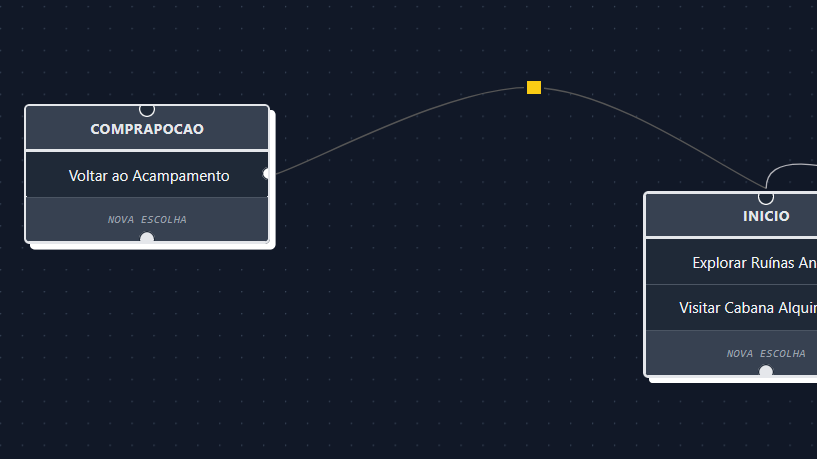
\includegraphics[width=0.65\textwidth]{Figures/curved_edge.png}
    \caption{Exemplo de aresta suavizada com caminho curvado personalizável no canvas.}
    \label{fig:curved-edge}
\end{figure}

O autor pode criar novos marcadores (\textit{waypoints}) com um duplo clique e arrastá-los livremente pelo ecrã. A curva é recalculada em tempo de execução à medida que os marcadores são movidos, interpolando a sua posição de forma contínua para manter a linha fluida e desimpedida de outros elementos do grafo.

\subsection{Acessibilidade e Identidade Visual Customizada}
\label{subsec:acessibilidade-identidade-visual}
Tendo em conta que o desenvolvimento do projeto beneficiou de validações diretas com utilizadores daltónicos, projetou-se uma estratégia de acessibilidade redundante baseada numa identidade visual neo-brutalista. A adoção desta estética neo-brutalista fundamentou-se em estudos que demonstram que contornos espessos, pesos tipográficos elevados e contrastes marcados beneficiam utilizadores com baixa acuidade visual ou daltonismo \citep{Babich2023, Loranger2022}. O aspeto geral desta interface e os seus elementos gráficos encontram-se representados na Figura~\ref{fig:editor-canvas-acessibilidade}.

\begin{figure}[H]
    \centering
    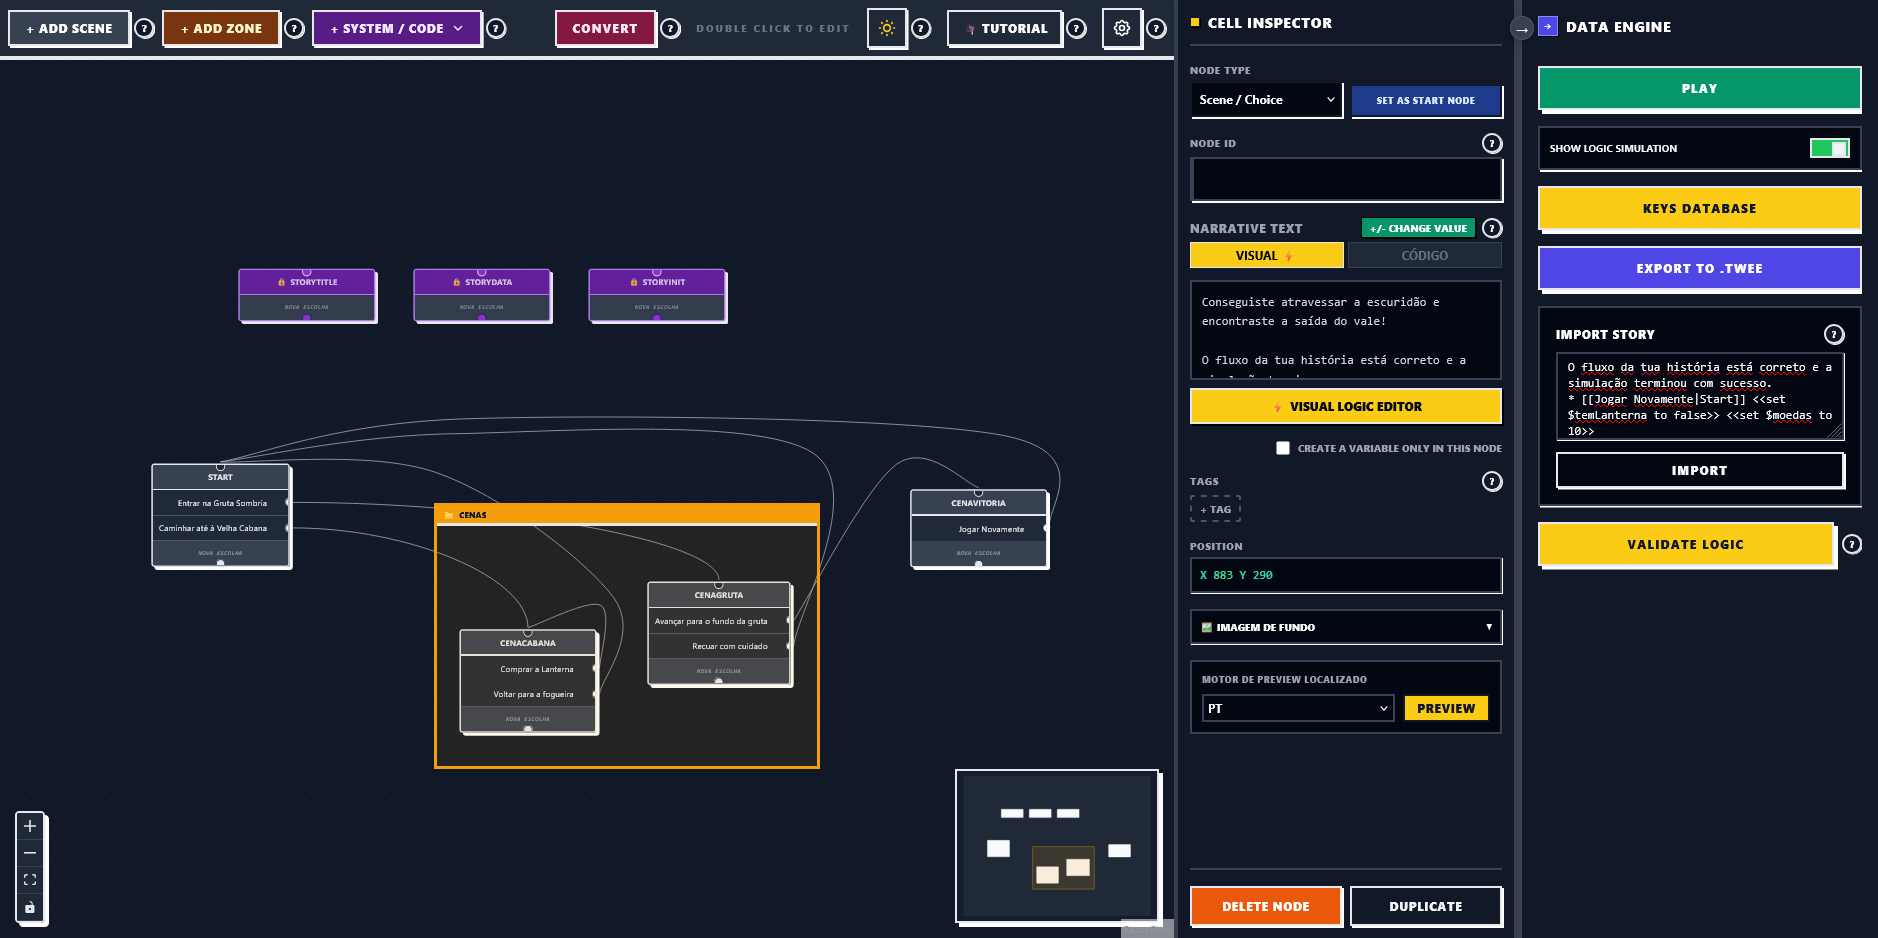
\includegraphics[width=0.85\textwidth]{Figures/editor_canvas.png}
    \caption{Interface gráfica global do editor (\textit{Plot in a Pot}), ilustrando a identidade visual neo-brutalista de alto contraste com contornos espessos e sinalização redundante para acessibilidade.}
    \label{fig:editor-canvas-acessibilidade}
\end{figure}

O nosso trabalho de design e programação focou-se nos seguintes pilares:
\begin{itemize}
    \item \textbf{Delimitação por Contornos Sólidos:} Implementação de contornos pretos de 2px (\texttt{border-2}) e sombras projetadas rígidas sem difusão (\texttt{shadow-[4px\_4px\_0px\_\#000]}) em todos os componentes visuais (\textit{StoryNode}, \textit{ZoneNode} e painéis), eliminando a dependência de cores ou gradientes suaves para distinguir elementos.
    \item \textbf{Diferenciação Estrutural de Arestas:} As transições normais no grafo são desenhadas com traçados contínuos, enquanto as ligações inacessíveis ou com erros lógicos são renderizadas com traçados tracejados (\texttt{strokeDasharray="5,5"}). Esta distinção de padrão garante que o utilizador consiga identificar caminhos quebrados sem depender exclusivamente da cor.
    \item \textbf{Sinalização Semântica Dupla de Alertas:} Configuração de etiquetas textuais explícitas (como o selo ``Aviso'' em fundo laranja nos nós com erros estruturais) em conjunto com listagens descritivas nos painéis, evitando a sinalização baseada apenas no par de cores verde/vermelho.
\end{itemize}

\subsection{Modelação de Dados e Sincronização com o React Flow}
\label{subsec:modelacao-dados-reactflow}
Para além da representação abstrata da arquitetura, a implementação prática exige uma sincronização bidirecional em tempo real entre a interface gráfica gerida pela biblioteca \textit{React Flow} e a estrutura de dados semântica interna da história.

No \gls{piap}, o estado centralizado da narrativa é mantido na raiz da aplicação (\texttt{App.jsx}) e de forma modular através de ganchos personalizados (\textit{custom hooks}), recorrendo a três vetores de dados estruturados em memória local:
\begin{enumerate}
    \item \textbf{Vetor de Nós do React Flow (\texttt{nodes}):} Contém a representação posicional e de renderização de cada elemento no canvas. Cada objeto de nó segue a especificação rígida da biblioteca:
\begin{verbatim}
{
  id: "cena_taberna",
  type: "storyNode",
  position: { x: 250, y: 180 },
  data: {
    title: "Interior da Taberna",
    content: "O cheiro a hidromel preenche a sala...",
    tags: ["secreto"],
    bgImage: ""
  },
  width: 280,
  height: 150
}
\end{verbatim}
    Se o nó representar uma Zona de Agrupamento (\texttt{ZoneNode}), o tipo é alterado para \texttt{"zoneNode"} e o objeto passa a incluir propriedades de agrupamento como \texttt{parentId} nos nós filhos e dimensões explícitas de largura e altura controladas pelo utilizador.
    
    \item \textbf{Vetor de Arestas do React Flow (\texttt{edges}):} Modela a conectividade geométrica das escolhas narrativas. Cada aresta é configurada como um componente personalizado (\texttt{EditableEdge}) e armazena os pontos geométricos intermédios (\textit{waypoints}) inseridos pelo autor para suavizar as curvas:
\begin{verbatim}
{
  id: "edge-cena_praca-cena_taberna",
  source: "cena_praca",
  target: "cena_taberna",
  type: "editableEdge",
  data: {
    choiceText: "Entrar na taberna",
    waypoints: [{ x: 120, y: 150 }, { x: 180, y: 160 }]
  }
}
\end{verbatim}
    
    \item \textbf{Lista de Adjacência Bidirecional (\texttt{adjacencyList}):} Representa o grafo direcionado de estados do ponto de vista do motor lógico. É recalculada de forma síncrona a cada modificação nos vetores de nós ou arestas. Esta lista mapeia cada identificador de cena ao seu conjunto de sucessores (saídas) e predecessores (entradas), permitindo ao validador e ao motor de simulação executar travessias e pesquisas rápidas.
\end{enumerate}

Esta tripla modelação é sincronizada de forma atómica. Quando o autor arrasta um nó ou altera o texto de uma escolha no painel de detalhes, os manipuladores de eventos reativos do React Flow (como \texttt{onNodesChange} ou \texttt{onEdgesChange}) capturam a alteração física. Esta alteração é processada e encaminhada pelos ganchos personalizados em \texttt{App.jsx}, gerando novos vetores imutáveis de estado que forçam a atualização dos componentes visuais e o recálculo imediato da lista de adjacências e do mapa de erros lógicos.

\section{Validação Estática e Simulação}
\label{sec:validacao-estatica-simulacao}

O motor de autoria do \textit{Plot in a Pot} integra ferramentas robustas de validação e execução reativa. Para além de permitir a escrita de histórias, a plataforma disponibiliza um sistema de verificação lógica que audita a estrutura narrativa de forma estática e uma sandbox de simulação dinâmica dotada de agentes de navegação autónoma.

\subsection{Algoritmo de Validação Estática e Exploração do Espaço de Estados (\gls{bfs})}
\label{subsec:algoritmo-bfs-validacao}

O validador estático, implementado em \texttt{storyValidator.js} e \texttt{storyTraversal.js}, resolve o problema de acessibilidade e integridade da narrativa. Em grafos estáticos simples, uma travessia clássica de Pesquisa em Largura (\gls{bfs}) seria suficiente para auditar o grafo. Contudo, em \gls{ni}, as arestas (hiperligações) dependem frequentemente de expressões lógicas e variáveis de estado (macros \texttt{<<if>>} e \texttt{<<set>>} do SugarCube). A acessibilidade de um nó $v$ não depende apenas do caminho geométrico, mas também da valoração atual das variáveis de estado (memória).

Assim, a validação lógica é modelada como um problema de \textit{Exploração do Espaço de Estados} (\textit{State Space Exploration}), onde o grafo de transições real é constituído por pares $\langle v, \sigma \rangle$, nos quais $v \in \mathcal{N}$ representa o nó do editor e $\sigma: \mathcal{V} \rightarrow \mathcal{D}$ representa um mapeamento de variáveis lógicas globais para os seus respetivos domínios de valores.

O algoritmo executa a travessia de acordo com os seguintes passos estruturados:

\begin{enumerate}
    \item \textbf{Inicialização e Pré-computação:}
    Para garantir a eficiência temporal ($\mathcal{O}(1)$ em lookups), o algoritmo pré-computa em memória:
    \begin{itemize}
        \item Um mapa de nós $NodeMap: \text{ID} \rightarrow Node$, indexando todos os vértices da narrativa.
        \item Um mapa de adjacências de arestas $EdgesBySource: \text{ID} \rightarrow List\langle Edge \rangle$.
    \end{itemize}
    O ponto de entrada $v_0$ é resolvido por $findStartNode(NodeMap)$, e o estado inicial $\sigma_0$ é lido a partir das declarações de variáveis do nó de sistema $StoryInit$.
    
    \item \textbf{Estrutura de Dados e Fila:}
    Uma fila síncrona $\mathcal{Q}$ é instanciada e inicializada com o tuplo de arranque:
    \[
    \mathcal{Q} \leftarrow \text{enqueue}\left(\mathcal{Q}, \langle v_0, \sigma_0, \text{path} = [v_0.\text{label}] \rangle\right)
    \]
    São criados conjuntos vazios para registar nós alcançáveis ($\mathcal{N}_{reach}$), arestas alcançáveis ($\mathcal{E}_{reach}$), e tabelas hash de estados visitados por nó ($VisitedStates: \text{ID} \rightarrow Set\langle String \rangle$) para evitar caminhos redundantes e ciclos infinitos.
    
    \item \textbf{Ciclo de Processamento Principal:}
    Enquanto $\mathcal{Q}$ não estiver vazia, remove-se o primeiro elemento:
    \[
    \langle u, \sigma, \text{path} \rangle \leftarrow \text{dequeue}(\mathcal{Q})
    \]
    Para o nó corrente $u$, efetua-se o seguinte processamento:
    \begin{enumerate}
        \item Adiciona-se o identificador de $u$ a $\mathcal{N}_{reach}$.
        \item Executam-se as instruções de modificação de estado contidas no texto do nó (por exemplo, macros de atribuição \texttt{<<set>>}), produzindo um novo estado de memória $\sigma' \leftarrow applyModifiers(u.\text{content}, \sigma)$.
        \item Verifica-se se o estado $\sigma'$ já foi visitado no nó $u$. Para tal, converte-se $\sigma'$ numa representação string serializada $S_{\sigma'}$ e verifica-se se $S_{\sigma'} \in VisitedStates[u]$. Em caso afirmativo, o ramo é podado (\textit{pruning}) para evitar ciclos redundantes no grafo.
        \item Para evitar a explosão do espaço de estados em loops que incrementam variáveis infinitamente, impõe-se um limite de segurança de $K = 10$ estados únicos por nó. Se $|VisitedStates[u]| \ge K$, o algoritmo emite um aviso de ciclo infinito no terminal e poda o caminho.
        \item Caso contrário, insere-se $S_{\sigma'}$ em $VisitedStates[u]$ e regista-se a rota percorrida e o estado final na tabela de histórico de chegada $ArrivalHistory[u]$.
    \end{enumerate}
    
    \item \textbf{Avaliação de Transições e Condicionais:}
    Para cada aresta de saída $e \in EdgesBySource[u]$ que conecta o nó $u$ ao nó de destino $w$:
    \begin{enumerate}
        \item O validador extrai a hiperligação textual associada à aresta $e$ do conteúdo de $u$.
        \item Avalia-se a condição de acessibilidade associada a essa escolha através da função $canAccessChoice(u.\text{content}, \text{link}, \sigma')$. Esta função analisa se o link está envolto por alguma macro condicional \texttt{<<if>>} e avalia a sua expressão lógica contra a memória $\sigma'$.
        \item Se a condição for satisfeita ($true$), adiciona-se o ID da aresta $e$ a $\mathcal{E}_{reach}$ e enfileira-se o próximo estado:
        \[
        \mathcal{Q} \leftarrow \text{enqueue}\left(\mathcal{Q}, \langle w, \sigma', \text{path} \cup [w.\text{label}] \rangle\right)
        \]
    \end{enumerate}
\end{enumerate}

Após o término da travessia (quando a fila $\mathcal{Q}$ fica vazia), o módulo de auditoria em \texttt{storyValidator.js} pós-processa os resultados recolhidos para isolar as falhas estruturais, categorizando-as em:
\begin{itemize}
    \item \textbf{Nós Órfãos ($V_{orphan}$):} Nós $v \in \mathcal{N}$ que não pertencem a $\mathcal{N}_{reach}$ e cujas etiquetas não incluem a tag \texttt{''secreto''}.
    \item \textbf{Becos sem Saída ($V_{dead\_end}$):} Nós $v \in \mathcal{N}_{reach}$ que contêm hiperligações cujo destino aponta para um ID de nó inexistente no grafo ($w \notin \mathcal{N}$).
    \item \textbf{Arestas Inacessíveis ($E_{unreachable}$):} Arestas $e \in \mathcal{E}$ que não pertencem a $\mathcal{E}_{reach}$. Estas representam caminhos cujas condicionais lógicas nunca são satisfeitas sob nenhuma das valorações de variáveis exploradas.
\end{itemize}

\subsection{Simulador em Tempo Real (PlayMode) e Smart Walker}
\label{subsec:simulador-playmode-walker}

O simulador de jogo (\texttt{PlayMode.jsx}) mimetiza o comportamento do interpretador SugarCube num ambiente controlado pelo navegador do autor. Para permitir a depuração em tempo real sem afetar os dados de edição, o motor executa sob um isolamento de contextos:
\begin{itemize}
    \item \textbf{Separação de Estilos:} Os nós categorizados com a tag \texttt{css} têm o seu conteúdo concatenado em tempo de execução e injetado sob a forma de uma tag \texttt{<style id=''playmode-styles''>} na raiz do cabeçalho da página, sendo totalmente limpos ao sair da simulação.
    \item \textbf{Isolamento de Scripts:} Os nós lógicos contendo JavaScript são processados como funções anónimas com escopo isolado através do construtor \texttt{new Function('state', 'State', 'setup', script\_content)}, impedindo que variáveis globais escritas pelo utilizador interfiram com os estados internos do React ou do canvas do React Flow.
\end{itemize}

Para testes automáticos de caminhos narrativos, a plataforma disponibiliza o agente autónomo \textbf{Smart Walker} (implementado em \texttt{storyTraversal.js}). Em vez de selecionar opções de forma puramente pseudo-aleatória (o que levaria a uma baixa cobertura de caminhos e retenção em ciclos curtos), o agente utiliza uma heurística baseada em \textit{Procura por Novidade} (\textit{Novelty Search}).

Dada a vizinhança do nó atual $v$, correspondente ao conjunto de nós adjacentes alcançáveis $N(v)$, o agente consulta o histórico de visitas acumuladas do simulador. Para cada opção de transição que leva ao nó vizinho $w \in N(v)$, o Smart Walker obtém o número acumulado de visitas históricas $H(w)$ registado na memória global do simulador. O Walker seleciona a transição para o nó vizinho $w_{next}$ que minimiza a frequência de visitas:
\[
w_{next} = \arg\min_{w \in N(v)} H(w)
\]
Este comportamento força o simulador a procurar caminhos narrativos raros e ramos profundos da história de forma automatizada, conseguindo mapear e encontrar becos sem saída ou ciclos lógicos fechados numa fração de segundo sem intervenção manual do autor.

\subsection{Motor de Compilação JIT de Macros SugarCube}
\label{subsec:compilador-jit-macros}

Para suportar as avaliações e atribuições de variáveis de estado descritas, a aplicação possui um compilador \textit{Just-In-Time} (JIT) simplificado estruturado em \texttt{logicParser.js} e \texttt{sugarcubeLogic.js}:
\begin{itemize}
    \item \textbf{Análise Léxica e Mapeamento:} O interpretador analisa o conteúdo textual dos nós através de varrimentos que procuram padrões de macros \texttt{<<set>>} e \texttt{<<if>>}. Traduz os operadores clássicos da linguagem SugarCube para os operadores lógicos válidos de JavaScript, conforme resumido na Tabela~\ref{tab:operadores-sugarcube}.
    \item \textbf{Árvore de Sintaxe Abstrata (\gls{ast}):} O interpretador de condicionais analisa blocos lógicos aninhados construindo uma \gls{ast} simples que reflete a precedência de cláusulas. Esta estrutura é então avaliada em tempo de execução para calcular o valor de verdade das expressões.
\end{itemize}

\begin{table}[htbp]
    \centering
    \caption{Mapeamento de operadores lógicos SugarCube para JavaScript.}
    \label{tab:operadores-sugarcube}
    \begin{tabular}{lll}
        \toprule
        \textbf{Operador SugarCube} & \textbf{Operador JavaScript} & \textbf{Significado} \\
        \midrule
        \texttt{is} / \texttt{eq} & \texttt{===} & Igualdade estrita \\
        \texttt{neq} & \texttt{!==} & Diferença estrita \\
        \texttt{and} & \texttt{\&\&} & E lógico \\
        \texttt{or} & \texttt{||} & OU lógico \\
        \texttt{to} & \texttt{=} & Atribuição de valor \\
        \texttt{\$variavel} & \texttt{state.variavel} & Acesso ao estado reativo \\
        \bottomrule
    \end{tabular}
\end{table}

\section{Integração de Modelos de Linguagem (LLMs)}
\label{sec:integracao-llms-implementacao}
Para além do núcleo lógico de grafos e da simulação estática, a plataforma disponibiliza um assistente baseado em Modelos de Linguagem de Grande Escala (LLMs) para facilitar a importação e co-criação de histórias. A conceção e implementação desta funcionalidade assenta nos seguintes aspetos:

\subsection{Arquitetura de Integração Local}
A integração com inteligência artificial foca-se em fornecer uma interface de comunicação local e assíncrona entre o editor gráfico e o servidor de inferência do utilizador. O trabalho de desenvolvimento realizado pela equipa consistiu em:
\begin{itemize}
    \item \textbf{Módulo de Comunicação REST (\texttt{aiGenerator.js}):} Programámos o cliente HTTP em Javascript para estabelecer a ligação assíncrona com o endpoint local do Ollama (\texttt{http://localhost:11434}), enviando os cabeçalhos e o corpo JSON com os parâmetros de temperatura e tokens.
    \item \textbf{Engenharia de Prompt de Conversão:} Desenvolvemos e validámos um prompt de sistema especializado, com regras sintáticas rígidas, concebido para forçar o modelo de linguagem a gerar respostas estritamente em conformidade com a especificação Twee 3 (cabeçalhos, metadados e arestas literais), mitigando alucinações.
    \item \textbf{Importação Automatizada Pós-Resposta:} Desenvolvemos o fluxo de importação que recebe o texto estruturado retornado pela API local, encaminha-o para o nosso parser e gera automaticamente os nós e arestas correspondentes no canvas.
\end{itemize}

A decisão de basear este assistente em inferência local (via Ollama) assenta nos seguintes compromissos:
\begin{itemize}
    \item \textbf{Privacidade e Soberania dos Dados:} Ao executar o modelo localmente no computador do autor, garante-se que toda a propriedade intelectual da história e os textos criados permanecem estritamente confidenciais. Não há partilha de dados com servidores externos de terceiros nem risco de os textos literários serem recolhidos para treino de modelos comerciais.
    \item \textbf{Custo Financeiro Zero:} APIs na nuvem implicam faturação contínua baseada em consumo de tokens, o que criaria barreiras ao uso regular. A inferência local permite a utilização gratuita e ilimitada da funcionalidade de conversão inteligente.
\end{itemize}

\subsection{Papel do LLM: Conversão e Importação Automática de Histórias}
A nossa abordagem de design delimitou de forma clara o papel do modelo de linguagem no ciclo de vida da narrativa. Visto que os LLMs tendem a alucinar, criar caminhos impossíveis e ignorar restrições de ciclos, o modelo não é integrado dinamicamente na simulação direta do jogo.

O papel do LLM foi desenhado por nós para atuar estritamente como uma ferramenta de conversão sintática em fase de pré-processamento. O modelo lê a história linear fornecida pelo autor e converte-a para a norma Twee 3. A partir desse ponto, o nosso motor lógico e o validador BFS assumem a responsabilidade exclusiva de renderizar o canvas visual e garantir a integridade dos caminhos e das variáveis de estado no editor.


